\documentclass[a4paper, 14pt, titlepage, fleqn]{extarticle}
\usepackage{style}
\usepackage{amsfonts}
\usepackage{float}
\usepackage{esint}
\usepackage{indentfirst}
\usepackage{setspace}
\usepackage{mathtools}
\usepackage{listings}
\DeclarePairedDelimiter\ceil{\lceil}{\rceil}
\DeclarePairedDelimiter\floor{\lfloor}{\rfloor}
\usepackage{color}


\definecolor{dkgreen}{rgb}{0,0.6,0}
\definecolor{gray}{rgb}{0.5,0.5,0.5}
\definecolor{mauve}{rgb}{0.58,0,0.82}

\lstset{frame=tb,
  language=C++,
  frame=single,
  aboveskip=3mm,
  belowskip=3mm,
  showstringspaces=false,
  columns=flexible,
  basicstyle={\small\ttfamily},
  numbers=none,
  keywordstyle=\color{blue},
  commentstyle=\color{dkgreen},
  stringstyle=\color{mauve},
  breaklines=true,
  breakatwhitespace=true,
  tabsize=1
}

\begin{document}
	\fefutitlepage{ОТЧЕТ}{к лабораторной работе №1\\по дисциплине <<Математическое моделирование>>}{01.03.02 <<Прикладная математика и информатика>>}{Б9120-01.03.02миопд}{Крюков Н.В.}
	\tableofcontents
	\newpage

    \onehalfspacing
    
    \sect{Введение}

        В данной лабораторной работе я буду решать задания, используя программы компьютерной математики. 
        Оформлять решенные задачи буду в среде компьютерной верстки <<\TeX>>, затем конвертировать в документ формата PDF.
        
    \sect{Задача о температуре нагревательного прибора}

        \subsect{Постановка задачи}
            Внезапно возникла потребность. 
            Стало необходимо узнать, как изменяется температура умного нагревательного прибора при условии всех теплопотерь. 
            Сам накревательный прибор может отключать часть своих нагревательных элементов при приближении к нужной температуре.
        
        \subsect{Выбор переменных}
            Множество нагревательных приборов и необходимых условий можно охарактеризовать конкретными параметрами
            
            \begin{enumerate}
                \item массой $m = 1 \ \text{килограмм}$;
                \item количеством нагревательных элементов в нагревательном приборе $n = 10 \ \text{шт}$
                \item мощностью $p = 3000 \ \text{Вт}$;
                \item материалом прибора - железо;
                \item удельной теплоёмкостью материала $c = 460 \ \dfrac{\text{Дж}}{\text{кг} \cdot \text{с}}$;
                \item коэффициентом конвективного теплообмена $k = 25 \ \dfrac{\text{Вт}}{\text{м}^2 \cdot \text{K}}$;
                \item площадью поверхности нагревательного прибора $S = 0.01 \ \text{м}^2$;
                \item температурой атмосферы $T_a = 300 \ \text{K}$;
                \item температурой, до которой необходимо нагреть нагревательный прибор $T_R = 600 \ \text{K}$.
            \end{enumerate}

            Также понадобится:

            Постоянная Стефана-Больцмана $\mathfrak{S} = 5.67 \cdot 10^{-8} \ \dfrac{\text{Вт}}{\text{м}^2 \cdot \text{K}^4}$.

        \subsect{Выбор законов и зависимостей}
            Для того, чтобы построить график изменения температуры, необходимо узнать, за счёт чего температура увеличивается и за счёт чего она может уменьшаться.
            При увеличении или уменьшении температуры количество тепла нагревательного прибора также увеличивается или уменьшается -- \( Q = c m T \) или же \( \Delta Q = c m \Delta T \).
            
            Уменьшение температуры может происходить по нескольким причинам: конвекция и тепловое излучение. 
            Формула конвективного теплообмена -- \( k S \left( T - T_a \right) \Delta t \).
            Формула теплового излучения -- \( S \mathfrak{S} \left( T^4 - T_a^4 \right) \Delta t \).
            Переобозачим суммарные потери как $L\left( T \right) \cdot \Delta t$.
            
            Увеличение количества тепла происходит за счёт мощности на единицу времени \(P \cdot \Delta t\).
            Предположим, что часть нагревательных элементов может отключаться, тогда домножим предыдущую формулу на некий коэффициент $H$, который будет меняться с изменениями температуры -- \( P \cdot \Delta t \cdot H \).
            
        \subsect{Формулировка математической модели}
            % Чтобы нагревательный прибор мог поддерживать 
        
            Узнаем сколько тепла получает и отдаёт нагревательный прибор
            \[ Q = P \cdot \Delta t \cdot H - L\left( T \right) \cdot \Delta t \]

            Подставим формулу количества тепла нагревательного элемента:
            \begin{equation}
                c m \Delta T = P \cdot \Delta t \cdot H - L\left( T \right) \cdot \Delta t
            \end{equation}

            Найдём функцию \(H\) 

            Чтобы нагревательный прибор поддерживал нужную температуру, необходимо узнать, сколько нагревательных элементов должно работать при необходимой температуре:
            Разделим теплопотери на мощность отдельно взятого нагревательного элемента:
            \[ \dfrac{L\left( T_R \right)}{\tfrac{P}{n}} = \dfrac{n \cdot L\left( T_R \right)}{P} \]

            Остальными нагревательными элементами мы можем распоряжаться свободно. Их количество:
            \[ n - \dfrac{n \cdot L\left(T\right)}{P} = n \cdot \left( 1 - \dfrac{L\left(T\right)}{P} \right) \]

            Допустим, чем ближе текущая температура к необходимой, тем меньше нагревательных элементов будет работать.
            Найдём в процентном соотношении количество оставшейся температуры:
            \[ \dfrac{T_R - T}{T_R - T_a} \]

            Так как значение этого выражения обычно находится на отрезке от 0 до 1, то извлечение корня из этого выражения только увеличит его.
            Это значит, что обычно будет работать больше нагревательных элементов, но при приближении к нужной температуре их количество будет быстро уменьшаться.
            Степень корня возьмём такую, что при различных начальных условиях температуры, нагрев происходил примерно за одно и то же время.
            \[ \left({\dfrac{T_R - T}{T_R - T_a}}\right)^{\tfrac{T_a}{T_R}} \] 
            
            Соберём функцию $H$
            \[ H = \left({\dfrac{T_R - T}{T_R - T_a}}\right)^{\tfrac{T_a}{T_R}} \cdot \left( 1 - \dfrac{L\left(T\right)}{P} \right) \cdot n + \dfrac{n \cdot L\left( T_R \right)}{P} \]
            
            Но так как в нашей модели невозможно, чтобы какой-то из нагревательных элементов работал на 0.5 от общей мощности, он либо включен, либо выключен, то округлим значение этого выражения вниз.
            А так же разделим результат на количество нагревательных элементов, чтобы получить процентное соотношение работающих элементов ко всем.
            \[ H = \dfrac { \floor*{\left({\dfrac{T_R - T}{T_R - T_a}}\right)^{\tfrac{T_a}{T_R}} \cdot \left( 1 - \dfrac{L\left(T\right)}{P} \right) \cdot n + \dfrac{n \cdot L\left( T_R \right)}{P}} }{n} \]

            Преобразуем уравнение $\left(1\right)$:
            \begin{equation}
                \dfrac{\Delta T}{\Delta t} = \dfrac{P \cdot H - L\left( T \right)}{c m}
            \end{equation}

            Математическая модель поставлена

        \subsect{Решение}

            Уравнение $\left(1\right)$ является дифференциальным уравнением температуры по времени.
            Так как в начальный момент времени $t_0$ температура равна атмосферной $T = T_a$, то значит эта задача является задачей Коши.
            Напишем программу для высчитывания графика роста температуры. 

        \subsect{Код программы}

    \begin{lstlisting}
    #include <iostream>
    #include <fstream>
    #include <cmath>
    #include <string>

    int m = 1;
    int p = 3000;
    int n = 100;
    int c = 460;
    int tA = 300;
    double k = 25;
    double s = 0.01;
    const double sigma = 5.7 * pow(10, -8);
    int tR = 600;

    using std::cin;
    using std::cout;
    using std::endl;
    using std::string;
    using std::ofstream;
    using std::to_string;

    double losses(double t) {
        return s * (k * (t - tA) + sigma * (pow(t, 4) - pow(tA, 4)));
    }

    double h(double t) {
        return 1.0 * floor(pow((((tR - t) > 0 ? (tR - t) : 0) * 1.0 / (tR - tA)), 1.0 * tA / tR) * (1 - losses(tR) / p) * n + n * losses(tR) / p);
    }

    double f(double t) {
        return (1.0 * (p * h(t) / n - losses(t)) / (c * m));
    }

    int main() {
        ofstream fout("output.txt");
        string x = "";
        string y = "";
        double t = tA;
        for (int i = 0; i < 100; i++) {
            cout << i << ' ' << h(t) << ' ' << t << ' ' << f(t) << endl;
            x += to_string(i);
            x += ", ";
            y += to_string(t);
            y += ", ";
            t += (double)f(t);
        }
        cout << "  " << n * losses(tR) / p << ' ' << losses(tR);
        fout << x << endl << y << endl;
        fout.close();
    }

    \end{lstlisting}

        \subsect{Тестирование}
            Проведём серию экспериментов

            Для визуализации результатов использовалась библиотека языка Python

            Первый эксперимент проведём с одним нагревательным элементом:
            \begin{figure}[H]
                \centering
                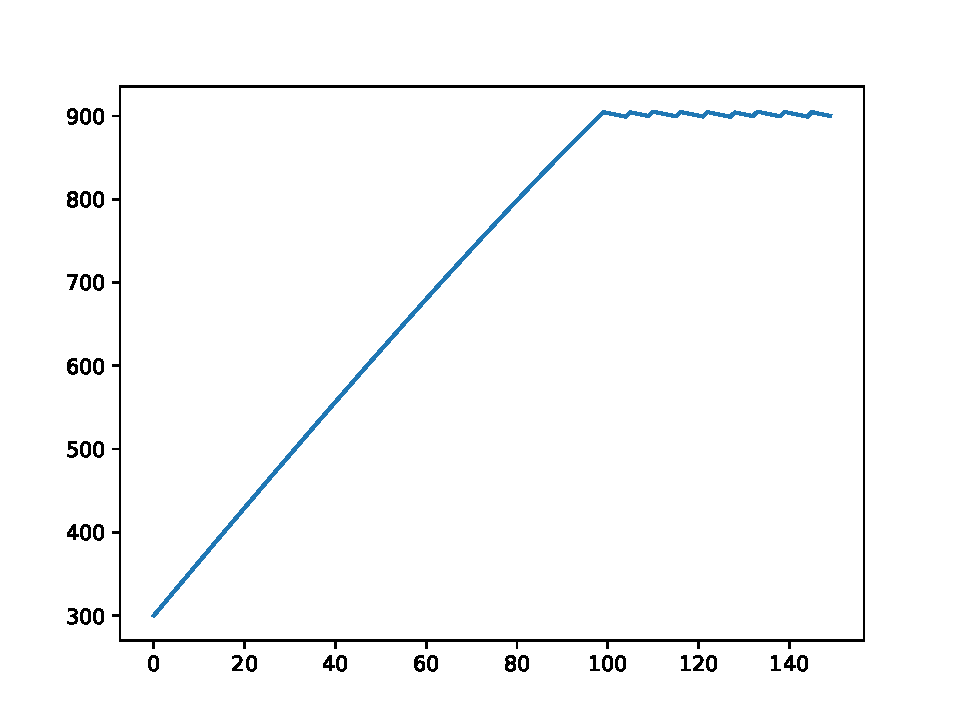
\includegraphics[width = .7\textwidth]{assets/n1t150T900.pdf}
                \caption[.] {График с одним нагревательным элементом}
            \end{figure}

            Второй эксперимент будет с пятью нагревательными элементами:
            \begin{figure}[H]
                \centering
                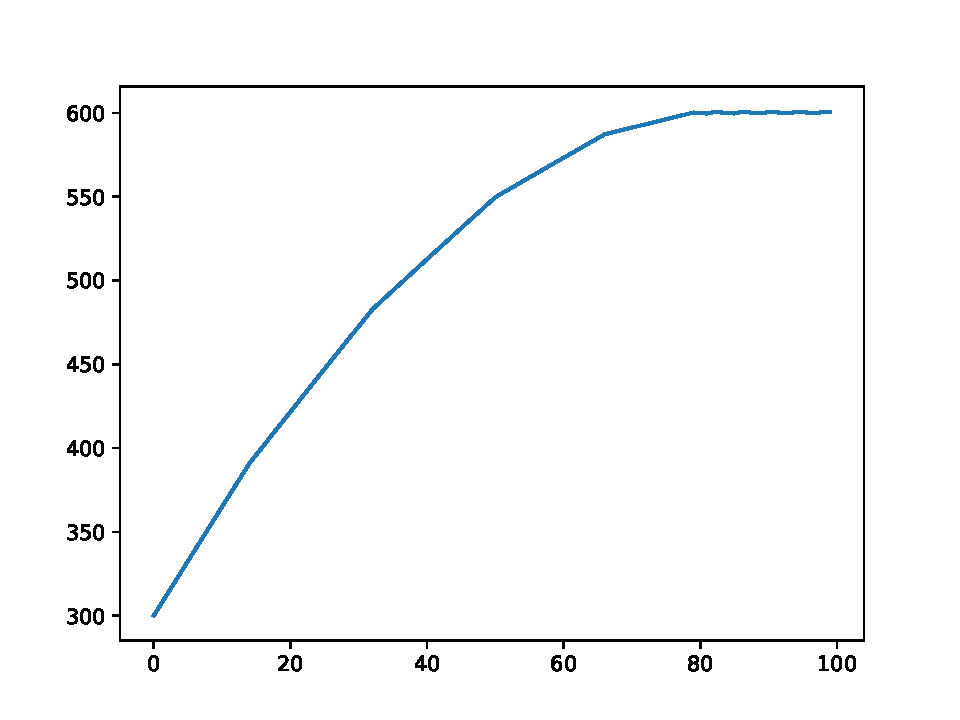
\includegraphics[width = .7\textwidth]{assets/n5t100T600.pdf}
                \caption[.] {График с пятью нагревательными элементами}
            \end{figure}

            Третий -- с десятью нагревательными элементами:
            \begin{figure}[H]
                \centering
                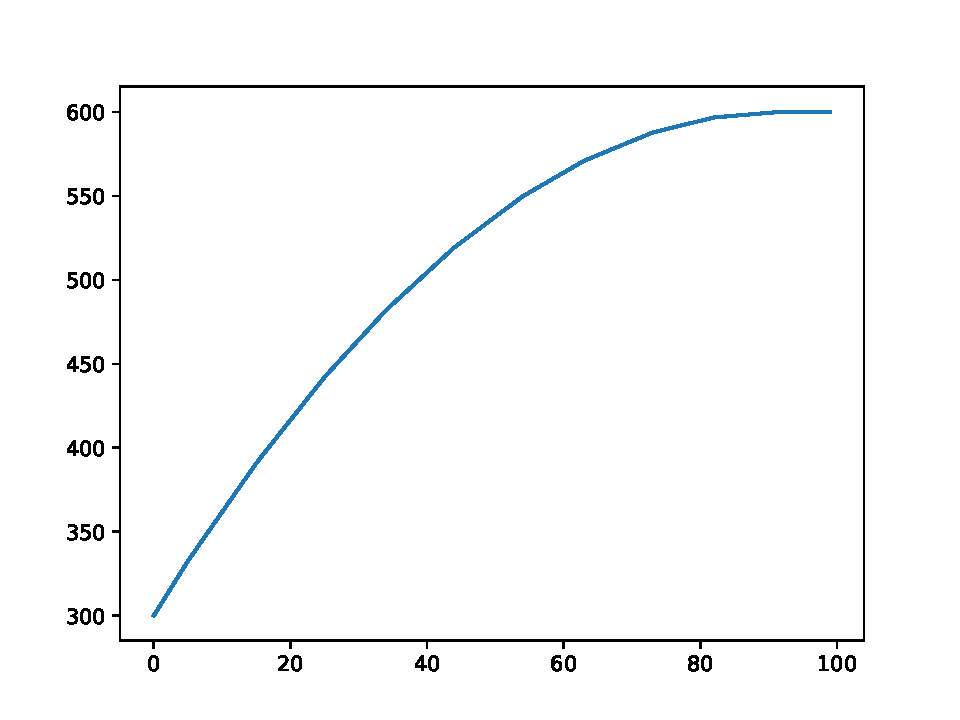
\includegraphics[width = .7\textwidth]{assets/n10t100T100.pdf}
                \caption[.] {График с десятью нагревательными элементами}
            \end{figure}            

    \sect{Заключение}
        
        В ходе работы была написана и протестирована программа для прогнозирования температуры нагревательного прибора с несколькими нагревательными элементами в своей конструкции. 

\end{document}